\iffalse
\let\negmedspace\undefined
\let\negthickspace\undefined
\documentclass[journal,12pt,twocolumn]{IEEEtran}
\usepackage{cite}
\usepackage{amsmath,amssymb,amsfonts}
\usepackage{graphicx}
\usepackage{textcomp}
\usepackage{xcolor}
\usepackage{txfonts}
\usepackage{listings}
\usepackage{enumitem}
\usepackage{mathtools}
\usepackage{gensymb}
\usepackage{comment}
\usepackage[breaklinks=true]{hyperref}
\usepackage{tkz-euclide} 
\usepackage{listings}
\usepackage{gvv}                                        
\def\inputGnumericTable{}                                 
\usepackage[latin1]{inputenc}                                
\usepackage{color}                                            
\usepackage{array}                                            
\usepackage{longtable}                                       
\usepackage{calc}                                             
\usepackage{multirow}                                         
\usepackage{hhline}                                           
\usepackage{ifthen}                                           
\usepackage{lscape}
\usepackage[export]{adjustbox}

\newtheorem{theorem}{Theorem}[section]
\newtheorem{problem}{Problem}
\newtheorem{proposition}{Proposition}[section]
\newtheorem{lemma}{Lemma}[section]
\newtheorem{corollary}[theorem]{Corollary}
\newtheorem{example}{Example}[section]
\newtheorem{definition}[problem]{Definition}
\newcommand{\BEQA}{\begin{eqnarray}}
	\newcommand{\EEQA}{\end{eqnarray}}
\newcommand{\define}{\stackrel{\triangle}{=}}
\newtheorem{rem}{Remark}

\begin{document}
	\parindent 0px
	\bibliographystyle{IEEEtran}
	
	
	\title{}
	\author{EE23BTECH11209 - K S Ballvardhan$^{*}$
	}
	\maketitle
	\newpage
	\bigskip
	
	% \renewcommand{\thefigure}{\theenumi}
	% \renewcommand{\thetable}{\theenumi}
	
	
	\section*{Exercise 9.5}
	
	\textbf{5.} Find the sum of integers from 1 to 100 that are divisible by 2 or 5.\\
	
	\solution
        \fi
	
	\begin{table}[ht]
		\centering
		\def\arraystretch{1.5}
		\begin{tabular}{|c|c|c|}
	\hline
	\textbf{Parameter} & \textbf{Value} & \textbf{Description} \\
	\hline
	$ x_1\brak{0}$ & 2 & First term \\
	\hline
	$ d_1$ & 2 & Common difference \\
	\hline
	$ x_1\brak{n}$ & [2+2n]u\brak{n} & General term of the series  \\
	\hline
	$ x_2\brak{0}$ & 5 & First term  \\
	\hline
	$ d_2$ & 10 & Common difference \\
	\hline
	$ x_2\brak{n}$ & [5+5n]u\brak{n} & General term of the series \\
	\hline
\end{tabular}
		\caption{Parameter Table1}
		\label{tab:10.5.3.1}
	\end{table}
	
	For an $AP$,
	\begin{align}
		X\brak z &= \frac{ x\brak 0 }{1-z^{-1}} + \frac{dz^{-1}}{{(1-z^{-1})}^{2}} 
    \end{align}
    By the problem there are two APs,
    \begin{align}
		\implies X\brak z &= \frac{2}{1-z^{-1}} + \frac{2z^{-1}}{{(1-z^{-1})}^{2}}
		+ \frac{5}{1-z^{-1}} + \frac{10z^{-1}}{{(1-z^{-1})}^{2}} \\
		&= \frac{2}{({1-z^{-1})}^{2}} + \frac{5+5z^{-1}}{({1-z^{-1})}^{2}}, \quad \abs{z}>1 \\
		y\brak{n}&=x\brak{n}\ast u\brak{n} \\
		\implies Y\brak{z}&=X\brak{z}U\brak{z} \\
		Y\brak{z}&=\brak{\frac{2}{({1-z^{-1})}^{2}} + \frac{5+5z^{-1}}{({1-z^{-1})}^{2}}}\brak{\frac{1}{1-z^{-1}}}\\
		&= \frac{2}{({1-z^{-1})}^{3}} + \frac{5+5z^{-1}}{({1-z^{-1})}^{3}},  \quad \abs{z}>1\\
		Y\brak{z}&= Y_1\brak{z} + Y_2\brak{z} 
	\end{align}
	Using Contour Integration to find the inverse $Z$-transform,
	\begin{align}
		y_1(49)&=\frac{1}{2\pi j}\oint_{C}Y_1(z) \;z^{48} \;dz  \\
		&=\frac{1}{2\pi j}\oint_{C}\frac{2z^{48}}{({1-z^{-1})}^{3}} \;dz 
	\end{align}
	\begin{align}
		y_2(9)&=\frac{1}{2\pi j}\oint_{C}Y_2(z) \;z^{8} \;dz  \\
		&=\frac{1}{2\pi j}\oint_{C}\frac{\brak{5+5z^{-1}}z^{8}}{({1-z^{-1})}^{3}} \;dz 
	\end{align}
	We can observe that the pole is repeated $3$ times and thus $m=3$,
	\begin{align}
		R_1&=\frac{1}{\brak {m-1}!}\lim\limits_{z\to a}\frac{d^{m-1}}{dz^{m-1}}\brak {{(z-a)}^{m}f\brak z}  \\
		&=\frac{1}{\brak {2}!}\lim\limits_{z\to 1}\frac{d^{2}}{dz^{2}}\brak {{(z-1)}^{3}\frac{2z^{51}}{{(z-1)}^3}}   \\
		&=\lim\limits_{z\to 1}\frac{d^2}{dz^2}(z^{51})   \\
		&=2550
	\end{align}
	\begin{align}
		R_2&=\frac{1}{\brak {2}!}\lim\limits_{z\to 1}\frac{d^{2}}{dz^{2}}\brak {{(z-1)}^{3}\frac{\brak{5z+5}z^{10}}{{(z-1)}^3}}   \\
		&=\frac{1}{{2}}\lim\limits_{z\to 1}\frac{d^2}{dz^2}(5z^{11}+5z^{10})   \\
		&=500
	\end{align}
	\begin{align}
		\therefore y(59)&= R_1 + R_2 \\
		 &= 2550 + 500\\
		 &= 3050
	\end{align}
	\begin{figure}[ht]
		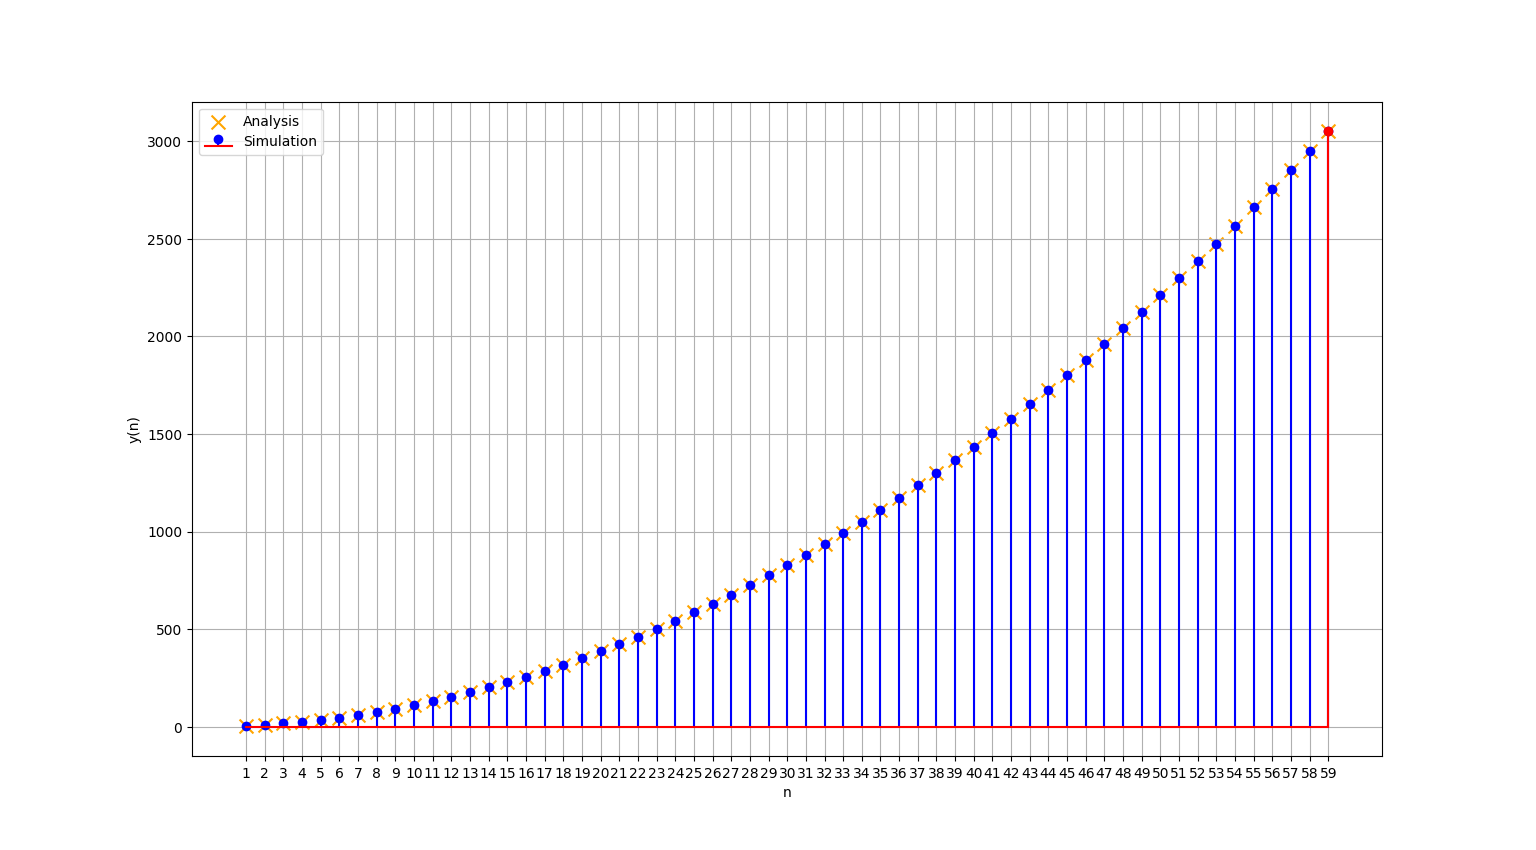
\includegraphics[width = \columnwidth]{ncert-maths/11/9/5/5/figs/fig1}
		\caption{y(n) vs n}
		\centering
		\label{fig: fig1}
	\end{figure}
%\end{document}
